\documentclass[tikz,border=6pt]{standalone}
\usepackage{fontspec}
\setmainfont{Noto Sans}
\usepackage{tikz}
\usetikzlibrary{arrows.meta,positioning}
\definecolor{cudaG}{RGB}{118,185,0}
\definecolor{gsBlue}{RGB}{40,110,190}
\definecolor{pyYel}{RGB}{240,170,30}
\definecolor{secG}{RGB}{85,85,85}
\begin{document}
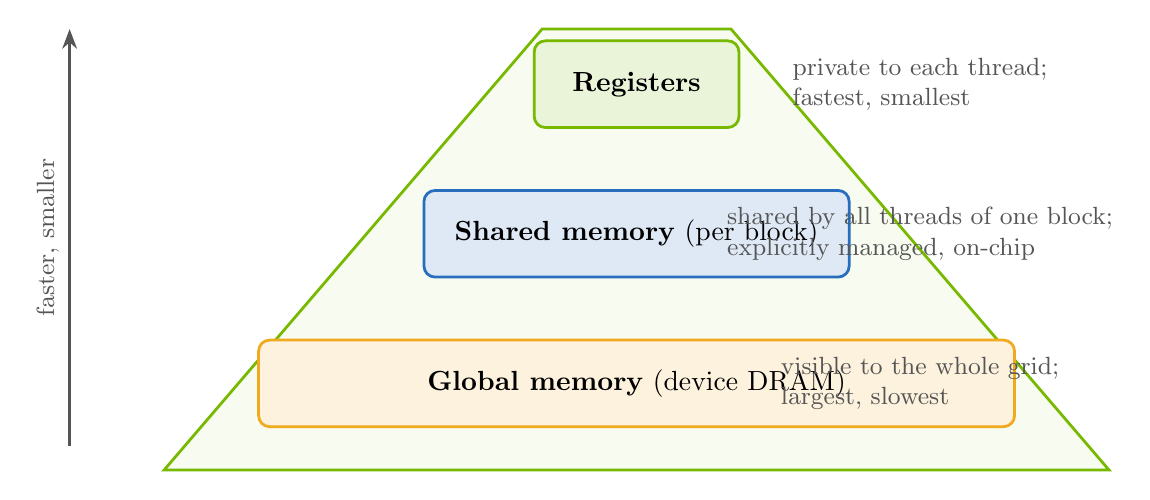
\begin{tikzpicture}[font=\sffamily]
  \tikzset{lay/.style={draw=#1,line width=1pt,fill=#1!15,align=center,minimum height=1.1cm,font=\normalsize,rounded corners}}
  % pyramid: wide base = global, narrow top = registers
  \draw[fill=cudaG!6,draw=cudaG,line width=1pt] (-6.0,0) -- (6.0,0) -- (1.2,5.6) -- (-1.2,5.6) -- cycle;
  \node[lay=cudaG,minimum width=2.6cm] at (0,4.9) {\textbf{Registers}};
  \node[lay=gsBlue,minimum width=5.4cm] at (0,3.0) {\textbf{Shared memory} (per block)};
  \node[lay=pyYel,minimum width=9.6cm] at (0,1.1) {\textbf{Global memory} (device DRAM)};
  \node[align=left,font=\small,secG] at (3.6,4.9) {private to each thread;\\fastest, smallest};
  \node[align=left,font=\small,secG] at (3.6,3.0) {shared by all threads of one block;\\explicitly managed, on-chip};
  \node[align=left,font=\small,secG] at (3.6,1.1) {visible to the whole grid;\\largest, slowest};
  \draw[-{Stealth[length=2.5mm]},line width=1pt,secG] (-7.2,0.3) -- (-7.2,5.6) node[midway,rotate=90,above,font=\small,secG] {faster, smaller};
\end{tikzpicture}
\end{document}
